\textbf{1. Input data.} The physical parameters are
\[
\boxed{L=0.85\,\mathrm{m},\qquad c=340\,\mathrm{m/s},\qquad \rho=1.2\,\mathrm{kg/m^3},\qquad N=5}.
\]
The corresponding acoustic bulk modulus is
\[
K=\rho c^2=1.2(340)^2\,\mathrm{Pa}\approx138.7\,\mathrm{kPa}.
\]
The boundary-condition derivations follow the course notes on pp.~109--123 and the closed--open and open--open developments in Problems C.1 and C.2. The harmonic displacement and pressure fields use $u(x,t)=U(x)e^{-i\omega t}$ and $p=-K\,u_x$. The displacement amplitude $a_j$ has units of meters.

\textbf{2(i). Closed--open tube.} The boundary conditions are
\[
u(0,t)=0,\qquad p(L,t)=0.
\]
With $U(x)=C_1\sin(\gamma x)+C_2\cos(\gamma x)$, the first condition gives $C_2=0$. The second condition then requires $C_1\cos(\gamma L)=0$. A nontrivial mode therefore satisfies
\[
\cos z=0,\qquad z=\gamma L,
\]
so that
\[
\boxed{z_j=\frac{(2j-1)\pi}{2}},\qquad
\boxed{\gamma_j=\frac{(2j-1)\pi}{2L}},\qquad
\boxed{\omega_j=c\gamma_j},\qquad
\boxed{f_j=\frac{\omega_j}{2\pi}=\frac{(2j-1)c}{4L}}.
\]
For the specified inputs, $c/L=400\,\mathrm{s^{-1}}$ and the first five modes are
\begin{table}[H]
\centering
\caption{Closed--open modal vibration characteristics.}
\label{tab:hw02-c3-closed-open}
\small
\begin{tabular}{@{}ccccc@{}}
\toprule
Mode $j$ & $z_j$ (rad) & $\gamma_j$ (rad/m) & $\omega_j$ (krad/s) & $f_j$ (Hz) \\
\midrule
1 & $\pi/2\approx1.571$ & $1.848$ & $0.628$ & $100$ \\
2 & $3\pi/2\approx4.71$ & $5.54$ & $1.885$ & $300$ \\
3 & $5\pi/2\approx7.85$ & $9.24$ & $3.14$ & $500$ \\
4 & $7\pi/2\approx11.00$ & $12.94$ & $4.40$ & $700$ \\
5 & $9\pi/2\approx14.14$ & $16.63$ & $5.65$ & $900$ \\
\bottomrule
\end{tabular}
\end{table}

\textbf{3(i). Displacement modeshapes.} Since $C_2=0$, setting the arbitrary displacement scale to one gives
\[
\boxed{U_j(x)=\sin(\gamma_jx)=\sin\left(\frac{(2j-1)\pi x}{2L}\right)},\qquad j=1,\ldots,5.
\]
The first five physical-length modeshapes are shown in Figure~\ref{fig:hw02-c3-closed-open-disp}.

\begin{figure}[H]
\centering
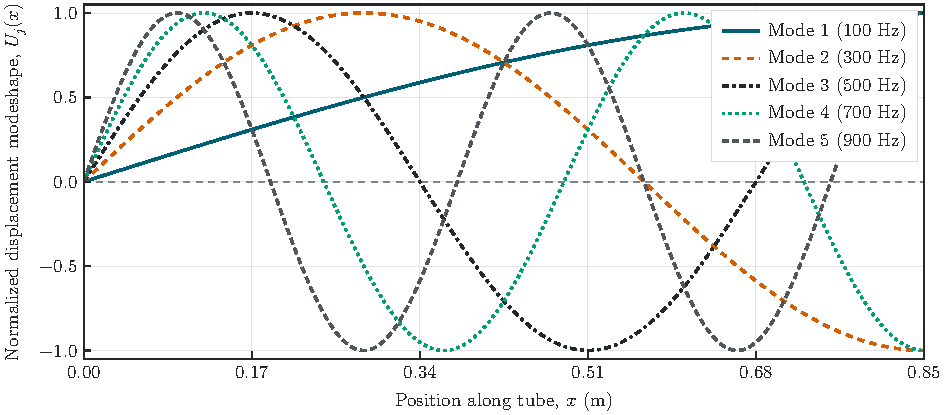
\includegraphics[width=0.96\linewidth]{figures/generated/solutions/C3-closed-open-displacement.pdf}
\caption{Closed--open displacement modeshapes for $L=0.85\,\mathrm{m}$. Legend frequencies identify the five modes.}
\label{fig:hw02-c3-closed-open-disp}
\end{figure}

\textbf{4(i). Comparison with B.4.} B.4 has $z_j=j\pi$ and $f_j=200j\,\mathrm{Hz}$. The closed--open fundamental is half as large, $100\,\mathrm{Hz}$, and only its odd harmonics occur. Both tubes have a displacement node and pressure antinode at $x=0$. Opening the right end replaces the B.4 displacement node with an antinode and its pressure antinode with a node.

The closed--open mode $j$ has $j$ displacement nodes including the closed end and $j$ antinodes including the open end. Its pressure field has $j$ nodes including the open end and $j$ antinodes including the closed end. B.4 instead has $j+1$ displacement nodes including both ends and $j$ interior antinodes; its pressure field has $j$ interior nodes and $j+1$ antinodes including both ends.

\textbf{5(i). Graduate work.} Let $a_j>0$ be the displacement amplitude in meters. Differentiating the displacement field in $p=-K u_x$ gives
\[
p_j(x,t)=-K a_j\gamma_j\cos(\gamma_jx)e^{-i\omega_jt}.
\]
Normalizing by the positive pressure scale $K a_j\gamma_j$ gives
\[
\boxed{\bar{P}_j(x)=-\cos(\gamma_jx)=-\cos\left(\frac{(2j-1)\pi x}{2L}\right)}.
\]
The normalized pressure modeshapes are shown in Figure~\ref{fig:hw02-c3-closed-open-pressure}. The pressure and displacement fields are quarter-cycle shifted because pressure is proportional to the negative spatial derivative of displacement. The closed end is a pressure antinode and displacement node, while the open end is a pressure node and displacement antinode.

\begin{figure}[H]
\centering
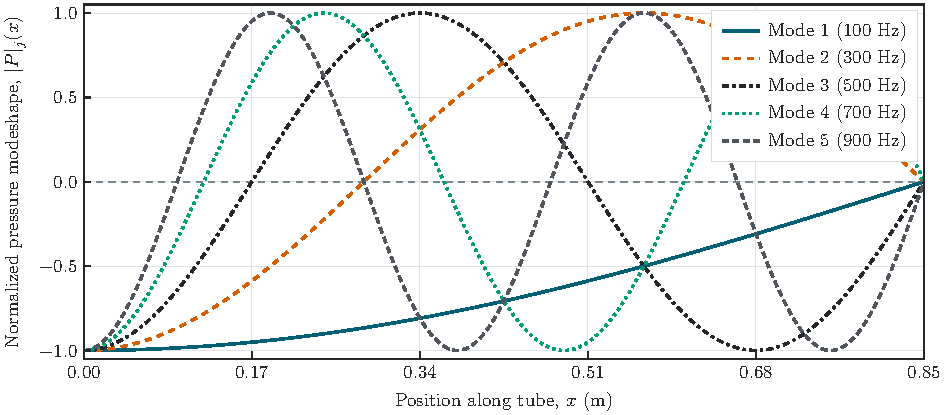
\includegraphics[width=0.96\linewidth]{figures/generated/solutions/C3-closed-open-pressure.pdf}
\caption{Closed--open normalized pressure modeshapes $\bar{P}_j(x)$ for $L=0.85\,\mathrm{m}$.}
\label{fig:hw02-c3-closed-open-pressure}
\end{figure}

\textbf{2(ii). Open--open tube.} The boundary conditions are
\[
p(0,t)=0,\qquad p(L,t)=0.
\]
The first condition gives $C_1=0$, and the second then requires $C_2\sin(\gamma L)=0$. The positive nontrivial roots are
\[
\boxed{z_j=j\pi},\qquad
\boxed{\gamma_j=\frac{j\pi}{L}},\qquad
\boxed{\omega_j=c\gamma_j},\qquad
\boxed{f_j=\frac{jc}{2L}}.
\]
The zero root is a rigid, zero-frequency displacement and is excluded from the acoustic mode index. The first five acoustic modes are
\begin{table}[H]
\centering
\caption{Open--open modal vibration characteristics.}
\label{tab:hw02-c3-open-open}
\small
\begin{tabular}{@{}ccccc@{}}
\toprule
Mode $j$ & $z_j$ (rad) & $\gamma_j$ (rad/m) & $\omega_j$ (krad/s) & $f_j$ (Hz) \\
\midrule
1 & $\pi\approx3.14$ & $3.70$ & $1.257$ & $200$ \\
2 & $2\pi\approx6.28$ & $7.39$ & $2.51$ & $400$ \\
3 & $3\pi\approx9.42$ & $11.09$ & $3.77$ & $600$ \\
4 & $4\pi\approx12.57$ & $14.78$ & $5.03$ & $800$ \\
5 & $5\pi\approx15.71$ & $18.48$ & $6.28$ & $1000$ \\
\bottomrule
\end{tabular}
\end{table}

\textbf{3(ii). Displacement modeshapes.} Since $C_1=0$, setting the arbitrary displacement scale to one gives
\[
\boxed{U_j(x)=\cos(\gamma_jx)=\cos\left(\frac{j\pi x}{L}\right)},\qquad j=1,\ldots,5.
\]
The first five physical-length modeshapes are shown in Figure~\ref{fig:hw02-c3-open-open-disp}.

\begin{figure}[H]
\centering
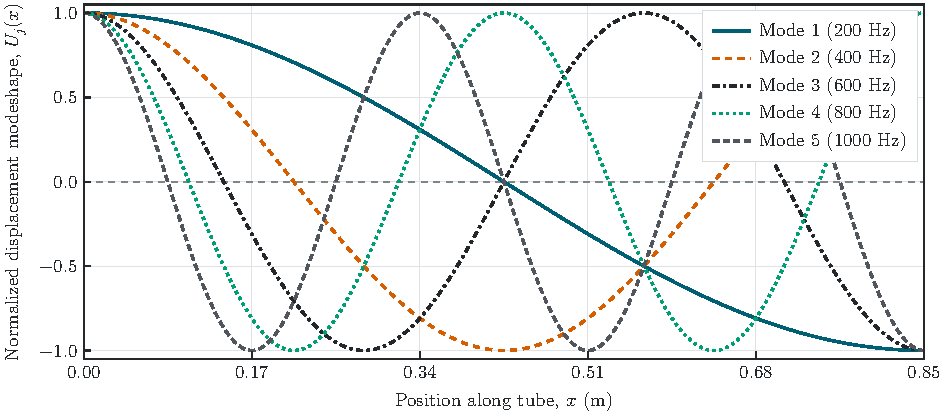
\includegraphics[width=0.96\linewidth]{figures/generated/solutions/C3-open-open-displacement.pdf}
\caption{Open--open displacement modeshapes for $L=0.85\,\mathrm{m}$. Legend frequencies identify the five modes.}
\label{fig:hw02-c3-open-open-disp}
\end{figure}

\textbf{4(ii). Comparison with B.4.} The open--open tube has the same eigenvalues, wavenumbers, and frequencies as B.4. Its cosine displacement and sine pressure shapes are shifted spatially by a quarter-wavelength from the B.4 sine displacement and negative-cosine pressure shapes. Both open ends are displacement antinodes and pressure nodes, reversing the B.4 endpoint roles.

Mode $j$ has $j$ interior displacement nodes and $j+1$ displacement antinodes including both ends. Its pressure field has $j+1$ nodes including both ends and $j$ interior antinodes. B.4 has $j+1$ displacement nodes including both ends and $j$ interior antinodes, with these counts reversed for pressure.

\textbf{5(ii). Graduate work.} Differentiating $U_j(x)$ gives
\[
p_j(x,t)=K a_j\gamma_j\sin(\gamma_jx)e^{-i\omega_jt}.
\]
Normalizing by the positive pressure scale $K a_j\gamma_j$ gives
\[
\boxed{\bar{P}_j(x)=\sin(\gamma_jx)=\sin\left(\frac{j\pi x}{L}\right)}.
\]
The normalized pressure modeshapes are shown in Figure~\ref{fig:hw02-c3-open-open-pressure}. The open ends are pressure nodes and displacement antinodes. The pressure field remains the spatial derivative relation $p=-K u_x$, so the positive sign follows from differentiating the cosine displacement shape.

\begin{figure}[H]
\centering
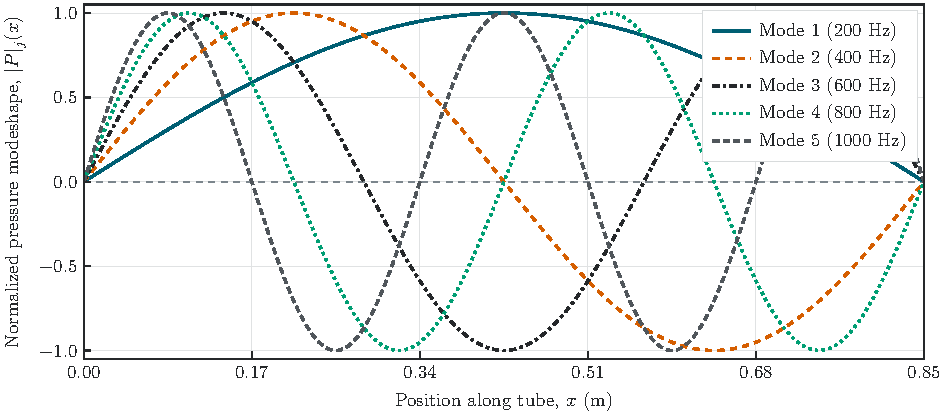
\includegraphics[width=0.96\linewidth]{figures/generated/solutions/C3-open-open-pressure.pdf}
\caption{Open--open normalized pressure modeshapes $\bar{P}_j(x)$ for $L=0.85\,\mathrm{m}$.}
\label{fig:hw02-c3-open-open-pressure}
\end{figure}

\clearpage
\matlabcaption{MATLAB calculations and plots for C.3.}
\lstinputlisting[style=hwmatlab]{matlab/C3.m}
